\documentclass[a4paper,12pt]{article}
\usepackage[T2A]{fontenc}
\usepackage[utf8]{inputenc}
\usepackage[english,russian]{babel}
\usepackage{listings}

\usepackage{amsmath}
\usepackage{MnSymbol}
\usepackage{wasysym}
\usepackage{indentfirst}

\usepackage{pgfplots}
\pgfplotsset{compat=1.9}

\usepackage{geometry}
\geometry{left=2cm}
\geometry{right=1.5cm}
\geometry{top=1cm}
\geometry{bottom=2cm}

\usepackage{graphicx}
\graphicspath{{img/}}
\DeclareGraphicsExtensions{.pdf,.png,.jpg}

\newcommand{\anonsection}[1]{\section*{#1}\addcontentsline{toc}{section}{#1}}

\lstset{
    language=C++,
    numbers=left,
    frame=single,
    texcl=true,
    basicstyle=\ttfamily
}

\begin{document}

\begin{titlepage}

    \begin{center}
        \large
        Государственное образовательное учреждение высшего профессионального образования\\
        “Московский государственный технический университет имени Н.Э.Баумана”
        \vspace{3cm}

        \textsc{Дисциплина: Анализ алгоритмов}
        \vspace{0.5cm}

        \textsc{Лабораторная работа №3}
        \vspace{3cm}

        {\LARGE ТРУДОЕМКОСТЬ СОРТИРОВОК}
        \vspace{3cm}

        Студент группы ИУ7-53,\\
        Степанов Александр Олегович
        \vfill
    \end{center}

    \begin{flushright}
        \begin{tabular}{l}
            Преподаватели:\\
            Строганов Юрий Владимирович\\
            Волкова Лилия Леонидовна
        \end{tabular}
    \end{flushright}

    \begin{center}

        2019 г.

    \end{center}

\end{titlepage}

\tableofcontents

\newpage
\anonsection{Введение}

\newpage
\section{Аналитическая часть}

\subsection{Описание задачи}

\subsection{Пути решения}

\subsection{Выводы}

\newpage
\section{Конструкторская часть}

\subsection{IDEF0}

\begin{center}
    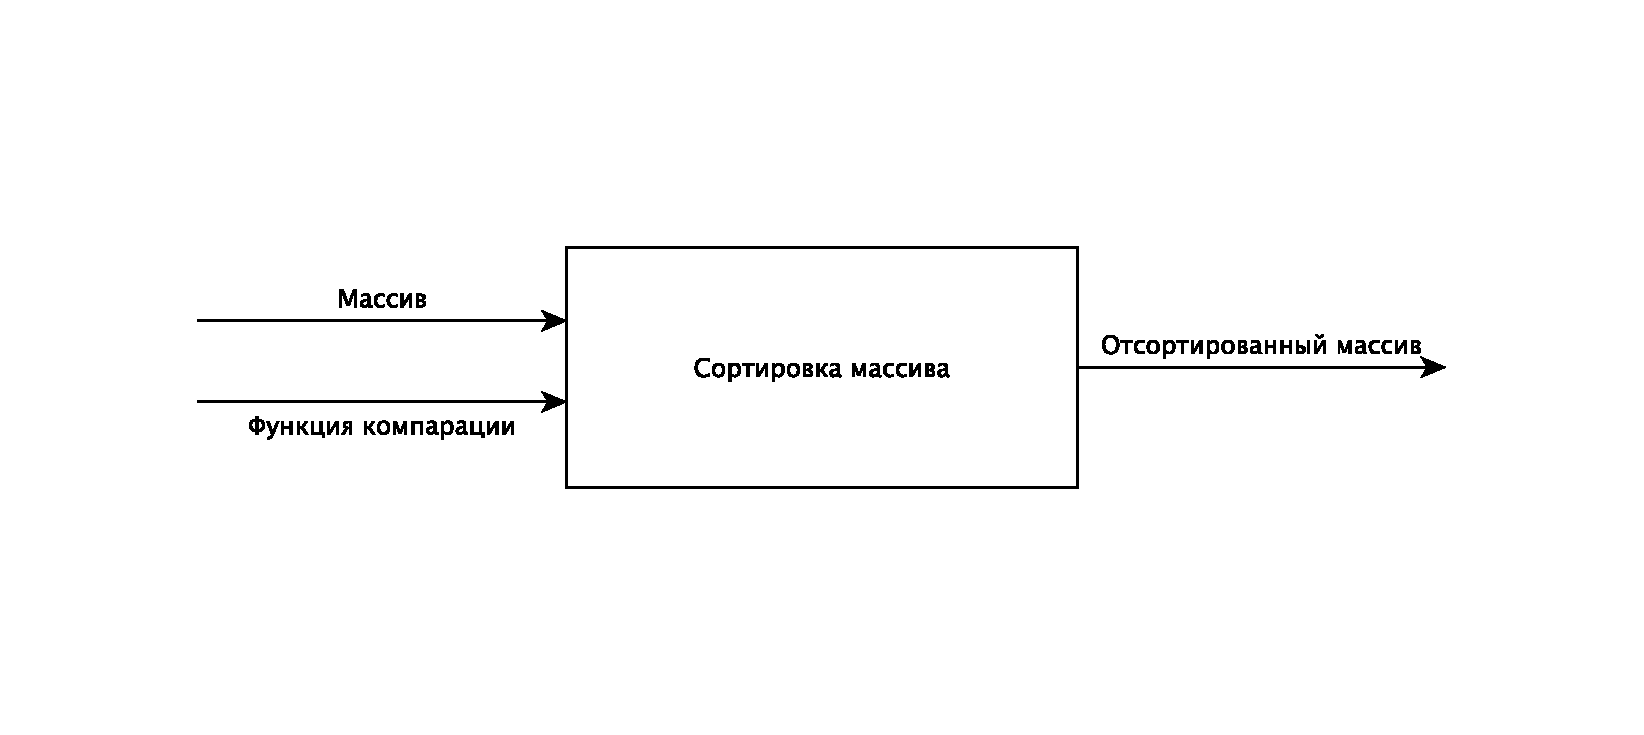
\includegraphics[scale=0.5]{IDEF0}
\end{center}

\subsection{Схемы алгоритмов}

\subsubsection{Сортировка пузырьком}

\begin{center}
    \includegraphics[scale=0.4]{Bubble}

    Схема 1. Сортировка пузырьком
\end{center}

\subsubsection{Сортировка шейкером}

\begin{center}
    \includegraphics[scale=0.5]{Shaker}

    Схема 2. Сортировка шейкером
\end{center}

\subsubsection{Быстрая сортировка}

\begin{center}
    \includegraphics[scale=0.45]{QSort}

    Схема 3. Быстрая сортировка
\end{center}

\subsection{Выводы}

\newpage
\section{Технологическая часть}

\subsection{Требования к программному обеспечению}

Программное обеспечение должно обеспечивать замер процессорного времени
выполнения каждого алгоритма. Проводятся замеры для случайно генерируемых
строк размерности до 1000. Выбранное ПО - MacOS.

\subsection{Средства реализации}

В качестве языка программирования был выбран C++. C++ компилируемый,
статически типизированный язык программирования общего назначения.
Данный язык имеет высокую скорость и богатую стандартную библиотеку,
содержащую необходимые контейнеры для данной работы, позволяющие
контролировать память благодаря объектно-ориентированному подходу
программирования.

\subsection{Листинг кода}

\begin{lstlisting}[caption=Сортировка пузырьком]
template < typename Type >
void BubbleSort< Type >::sort(std::vector< Type >& array,
                              bool (*comp)(Type, Type))
{
    for (int i = 0; i < array.size(); ++i) {
        for (int j = 0; j < array.size() - i - 1; ++j) {
            if (comp(array[j], array[j + 1])) {
                std::swap(array[j], array[j + 1]);
            }
        }
    }
}
\end{lstlisting}

\begin{lstlisting}[caption=Сортировка шейкером]
template < typename Type >
void ShakerSort< Type >::sort(std::vector< Type >& array,
                              bool (*comp)(Type, Type))
{
    int left = 0;
    int right = array.size() - 1;

    while (left <= right) {
        for (int i = left; i < right; ++i) {
            if (comp(array[i], array[i + 1])) {
                std::swap(array[i], array[i + 1]);
            }
        }
        --right;

        for (int i = right; i > left; --i) {
            if (comp(array[i - 1], array[i])) {
                std::swap(array[i - 1], array[i]);
            }
        }
        ++left;
    }
}
\end{lstlisting}

\begin{lstlisting}[caption=Быстрая сортировка]
template < typename Type >
void QSort< Type >::recursive(std::vector< Type >& array,
                              int start, int finish,
                              bool (*comp)(Type, Type))
{
    if (start < finish) {
        int left = start, right = finish;
        Type middle = array[(left + right) >> 1];

         while (left <= right) {
            while (comp(middle, array[left])) left++;
            while (comp(array[right], middle)) right--;

            if (left <= right) {
                std::swap(array[left], array[right]);
                ++left;
                --right;
            }
        }

        if (start < right) recursive(array, start, right, comp);
        if (left < finish) recursive(array, left, finish, comp);
    }
}
\end{lstlisting}

\subsection{Тестирование}

Для тестирования программы были заготовлены следующие тесты

\subsection{Выводы}

Для сравнения были реализованы 3 алгоритма на выбранном языке
программирования C++. Чтобы проверить правильность работы алгоритмов
были подготовлены тесты.

\newpage
\section{Экспериментальная часть}

\subsection{Примеры работ}

\subsection{Результаты тестирования}

\subsection{Замеры времени}

\begin{tikzpicture}
    \begin{axis}[
        title = Отсортированный массив,
        legend pos = north west,
        xlabel=size,
        ylabel=ms,
        grid = major,
        width = 0.8\paperwidth,
        height = 0.38\paperheight,
        line width = 1
    ]
        \legend{
            Сортировка пузырьком,
            Сортировка шейкером,
            Быстрая сортировка
        };
        \addplot[black] coordinates {
            (1000, 7293)
            (2000, 26795)
            (3000, 50656)
            (4000, 84619)
            (5000, 149956)
            (6000, 488432)
            (7000, 364641)
            (8000, 345024)
            (9000, 431258)
            (10000, 519986)
        };

        \addplot[dashed] coordinates {
            (1000, 6190)
            (2000, 23881)
            (3000, 48369)
            (4000, 68502)
            (5000, 125622)
            (6000, 172631)
            (7000, 220285)
            (8000, 266213)
            (9000, 342582)
            (10000, 418948)
        };

        \addplot[dotted] coordinates {
            (1000, 91)
            (2000, 207)
            (3000, 350)
            (4000, 294)
            (5000, 612)
            (6000, 478)
            (7000, 879)
            (8000, 619)
            (9000, 1157)
            (10000, 823)
        };
    \end{axis}
\end{tikzpicture}

\begin{tikzpicture}
    \begin{axis}[
        title = Обратно отсортированный массив,
        legend pos = north west,
        xlabel=size,
        ylabel=ms,
        grid = major,
        width = 0.8\paperwidth,
        height = 0.38\paperheight,
        line width = 1
    ]
        \legend{
            Сортировка пузырьком,
            Сортировка шейкером,
            Быстрая сортировка
        };
        \addplot[black] coordinates {
            (1000, 10910)
            (2000, 44509)
            (3000, 103662)
            (4000, 196315)
            (5000, 341381)
            (6000, 422604)
            (7000, 561695)
            (8000, 803356)
            (9000, 1093804)
            (10000, 1567691)
        };

        \addplot[dashed] coordinates {
            (1000, 14754)
            (2000, 55665)
            (3000, 132742)
            (4000, 184741)
            (5000, 264980)
            (6000, 374224)
            (7000, 505727)
            (8000, 660852)
            (9000, 809728)
            (10000, 987086)
        };

        \addplot[dotted] coordinates {
            (1000, 256)
            (2000, 214)
            (3000, 386)
            (4000, 479)
            (5000, 1688)
            (6000, 990)
            (7000, 1507)
            (8000, 1769)
            (9000, 778)
            (10000, 900)
        };
    \end{axis}
\end{tikzpicture}

\begin{tikzpicture}
    \begin{axis}[
        title = Случайный массив (среднее по 10 экспериментам),
        legend pos = north west,
        xlabel=size,
        ylabel=ms,
        grid = major,
        width = 0.8\paperwidth,
        height = 0.38\paperheight,
        line width = 1
    ]
        \legend{
            Сортировка пузырьком,
            Сортировка шейкером,
            Быстрая сортировка
        };
        \addplot[black] coordinates {
            (1000, 10534)
            (2000, 72452)
            (3000, 103098)
            (4000, 182016)
            (5000, 288249)
            (6000, 422482)
            (7000, 555036)
            (8000, 726603)
            (9000, 902156)
            (10000, 1132846)
        };

        \addplot[dashed] coordinates {
            (1000, 9510)
            (2000, 36276)
            (3000, 78982)
            (4000, 144617)
            (5000, 220086)
            (6000, 344491)
            (7000, 446781)
            (8000, 595689)
            (9000, 706823)
            (10000, 1019054)
        };

        \addplot[dotted] coordinates {
            (1000, 285)
            (2000, 560)
            (3000, 815)
            (4000, 1170)
            (5000, 1163)
            (6000, 1392)
            (7000, 1876)
            (8000, 2531)
            (9000, 2357)
            (10000, 2764)
        };
    \end{axis}
\end{tikzpicture}

\subsection{Выводы}


\newpage
\anonsection{Заключение}

\newpage
\anonsection{Список использованной литературы}
\end{document}
